\section{Approach} 
\label{approach}

\subsection{Reinforcement Learning Method and Regression Model} 
\label{ch:approachA}

% TODO: The first section shall describe the reinforcement learning method and regression model you finally implemented, including all crucial design choices. You may also describe approaches you tried and abandoned later, including the reasons.

\subsubsection{Features}
\label{ch:approachAa}

This chapter describes how the game state is transformed into input features for the model. 
Our initial encoding is based on \cite{Kormelink2018}. The Dictionary containing the game state is transformed into one vector, containing the input features.
Our input feature vector consists of the following five independent matrices:
\begin{itemize}
	\item Field state: free (0), breakable (1), obstructed cell (-1)
	\item Player position: player (1), otherwise(0)
	\item Opponent positions: opponent (1), otherwise(0)
	\item Danger level of position: danger (1), no danger (0) \newline
	Danger is caused by bombs on all fields an explosion can reach. Two aspects influence the value how dangerous a field is. The time until the bomb explodes and the distance from the bomb. We derived following equation for calculating the danger of a field for the field containing the bomb and the surrounding fields.
	
	$ danger = \frac{\frac{time\_Passed}{time\_needed\_to\_explode}}{\sqrt{distance}} $
	
	For example the bomb explodes after 4 time steps. Currently 2 time steps are over and the distance to the bomb is 3:
	
	$ danger = \frac{\frac{2}{4}}{\sqrt{2}} = 0.70 $
	
	TODO: normalized through equation
	TODO: advantage: gradation
	
	\item Desirability of position: desirable (1), not desirable (0)
\end{itemize}
These matrices are flattened and concatenated. This results in a feature vector containing 1445 elements (5*17*17).

Among other factors due to the high dimensionality the training process could be very slow. That is why the input state is further minimized.

TODO: adapt
\begin{itemize}
	\item Field state: free (0), breakable (1), obstructed cell (-1)
	\item Player position: player (1), otherwise(0)
	\item Opponent positions: opponent (1), otherwise(0)
	\item Danger level of position: danger (1), no danger (0)
	\item Desirability of position: desirable (1), not desirable (0)
\end{itemize}
These matrices are flattened and concatenated. This results in a feature vector containing 578 elements (2*17*17).


\subsubsection{Double dueling DQN}
\label{ch:approachAb}



\subsection{Training process} 
\label{ch:approachB}

% TODO: The second section should describe your training process, including all tricks employed to speed it up (e.g. self play strategy, design of auxilliary rewards, prioritization of experience replay and so on).

\subsubsection{Exploration-Exploitation}
\label{ch:approachBa}

When choosing the right method for the exploration-exploitation tradeoff, \cite{Kormelink2018} gives an insight in how different exploration methods perform in the Bomberman environment (see \autoref{fig:exploration}). 

\begin{figure}[ht]
	\centering
	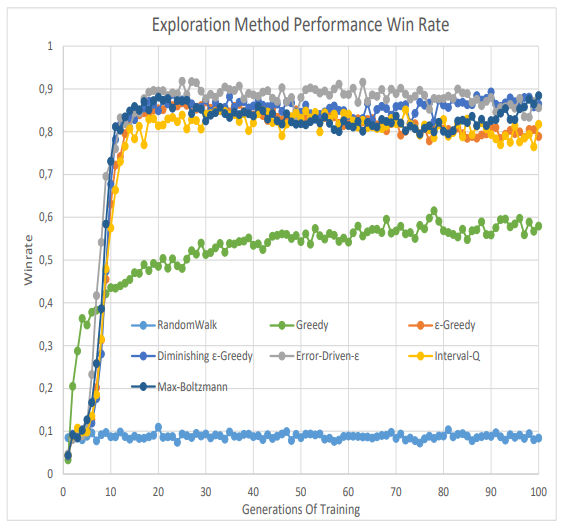
\includegraphics[width=0.6\linewidth]{figures/exploration.PNG}
	\caption{Comparison of different exploration methods}
	\label{fig:exploration}
\end{figure}

In the long run, Max Boltzmann performs best with 

\begin{equation}
	\Pi(s,a) = \frac{e^{Q(s,a)/T}}{\sum_i^{\abs{A}}e^{Q(s,a^i)/T}}
\end{equation}

and T being the temperature parameter. But as the result is based on 100 generations of training with each generation comprising 10.000 episodes, Diminishing $\epsilon$-Greedy as the second best exploration method was chosen as this exploration method converges faster in the early stages of training.

Two improvements where considered to optimize the exploration phase, but were discarded in the end. The first one is to replace the uniform sampling method by a multinomial sampling method in case an exploration step should be done, i.e. when a randomly generated number is smaller than $\epsilon$. This means the second best action would be chosen more often compared to other actions during the exploration phase. This could be beneficial especially in later phases of training in case the Q-values are close to each other. But esspecially in the beginning of the training phase this could lead towards an unintended bias towards specific actions as the exploration of others will be suppressed probabilistically.

The second improvement was to include an exploration function as \cite{Geron2018} proposes. A simple exploration function could be 

\begin{equation}
	f(q,n) = q + \frac{K}{1+n}
\end{equation}

with $q$ being the Q-value and $n$ being the count how often a specific action $a$ was chosen in state $s$. $K$ is a hyperparameter that determines the amount of curiosity during training. To implement this one would need to store $n$ for every state and action. But as the state is far too high dimensional in the Bomberman environment this would require a lot of training just as using the Max Boltzmann exploration method to be beneficial in the end. 

\subsubsection{Experience buffer and sum tree}
\label{ch:approachBb}

\subsubsection{Imitation learning}
\label{ch:approachBc}

\subsubsection{Rewards}
\label{ch:approachBd}

\subsubsection{Hyperparameters}
\label{ch:approachBe}

\subsubsection{Cloud training}
\label{ch:approachBf}

